\documentclass[onecolumn, draftclsnofoot,10pt, compsoc]{IEEEtran}
\usepackage{graphicx}
\usepackage{url}
\usepackage{setspace}
\usepackage{abstract}
\usepackage{geometry}
\geometry{textheight=9.5in, textwidth=7in}
\parindent = 0.0 in
\parskip = 0.1 in

% 1. Fill in these details
\def \CapstoneTeamName{WebXR Team}
\def \CapstoneTeamNumber{47}
\def \GroupMemberOne{Jonathan Jones}
\def \GroupMemberTwo{Evan Brass}
\def \GroupMemberThree{Brooks Mikkelsen}
\def \GroupMemberFour{Tim Forsyth}
\def \GroupMemberFive{Brandon Mei}
\def \CapstoneProjectName{Creating Immersive Experiences on the Web using VR and AR}
\def \CapstoneSponsorCompany{Intel}
\def \CapstoneSponsorPerson{Alexis Menard}

% 2. Uncomment the appropriate line below so that the document type works
\def \DocType{		        %Problem Statement
				%Requirements Document
				Technology Review
				%Design Document
				%Progress Report
				}
			
\newcommand{\NameSigPair}[1]{\par
\makebox[2.75in][r]{#1} \hfil 	\makebox[3.25in]{\makebox[2.25in]{\hrulefill} \hfill		\makebox[.75in]{\hrulefill}}
\par\vspace{-12pt} \textit{\tiny\noindent
\makebox[2.75in]{} \hfil		\makebox[3.25in]{\makebox[2.25in][r]{Signature} \hfill	\makebox[.75in][r]{Date}}}}
% 3. If the document is not to be signed, uncomment the RENEWcommand below
%\renewcommand{\NameSigPair}[1]{#1}

%%%%%%%%%%%%%%%%%%%%%%%%%%%%%%%%%%%%%%%
\begin{document}
\begin{titlepage}
    \pagenumbering{gobble}
    \begin{singlespace}
    	%\includegraphics[height=4cm]{coe_v_spot1}
        \hfill 
        % 4. If you have a logo, use this includegraphics command to put it on the coversheet.
        %\includegraphics[height=4cm]{CompanyLogo}   
        \par\vspace{.2in}
        \centering
        \scshape{
            \huge CS Capstone \DocType \par
            {\large\today}\par
            \vspace{.5in}
            \textbf{\Huge\CapstoneProjectName}\par
            \vfill
            {\large Prepared for}\par
            \Huge \CapstoneSponsorCompany\par
            \vspace{5pt}
            {\Large\NameSigPair{\CapstoneSponsorPerson}\par}
            {\large Prepared by }\par
            Group \CapstoneTeamNumber - WebPhysicsVR\par
            % 5. comment out the line below this one if you do not wish to name your team
            %\CapstoneTeamName\par 
            \vspace{5pt}
            {\Large
                \NameSigPair{\GroupMemberOne}\par
                \NameSigPair{\GroupMemberTwo}\par
                \NameSigPair{\GroupMemberThree}\par
                \NameSigPair{\GroupMemberFour}\par
                \NameSigPair{\GroupMemberFive}\par
            }
            \vspace{20pt}
        }
        %\renewcommand{\abstracttextfont}{\sffamily}
        \begin{abstract}
        % 6. Fill in your abstract
        This document is a technical review of researching different web hosting technologies options for the group 47 - WebPhysicsVR team's as a foundation. It will include the web hosting typed used for web pages to be viewed via the internet. This document outlines the Hosting and Publishing, Types of Web Hosting Technologies, and Content Delivery Network for the WebPhysicsVR. The site will then be deploy immersive web experience hosted by the Intel 01.org open source portal.
        \end{abstract}     
    \end{singlespace}
\end{titlepage}
\newpage
\pagenumbering{arabic}
\tableofcontents
% 7. uncomment this (if applicable). Consider adding a page break.
%\listoffigures
%\listoftables
\clearpage

% 8. now you write!
\section{Introduction}
\subsection{Purpose}
The purpose of this project is to provide a technical demonstration of the WebXR API capabilities. It will be an example of how WebXR can be used to create an entertaining, interactive VR experience within a web browser. It will have a focus on education and act as a virtual physics lab.

\subsection{Scope}
WebPhysicsVR will be an interactive physics simulation that utilizes the WebXR API. Its primary use is as tech demo and a platform for education.

As a tech demo, our project will incorporate all the major features of WebXR. We'll want to faithfully present the physical concepts in an educational and engaging fashion while also focusing on designing a quality WebXR experience.  

At a minimum, users should be able to visualize the effects of gravity.  If we have time to do so, we could visualize other forces like adding friction between objects or giving certain objects magnetism as well as mass.  

We intend to support a spectrum of VR devices though we will only test on a few selected devices that we have access to.
\subsection{Product overview}
%\subsubsection{Perspective}
\subsubsection{User Interfaces}
Users with compatible hardware will be able to experience an immersive/enhanced version of the website right when they access it, with a click of a button.

Within the VR experience, we will have interfaces for the user to manipulate the objects and physical constants. These interfaces will be displayed in the most contextually meaningful location in the environment.  This might mean different floating icons around the 3d objects, floating interfaces or control objects that are within the environment.

\subsubsection{Hardware Interfaces}
WebXR is compatible with a range of XR devices, web browsers and operating systems. This includes mobile devices. For the full intended experience, an HMD with body and controller tracking devices should be used.

\subsubsection{Software Interfaces}
\begin{itemize}
    \item WebXR API
    \item WebGL 2.0
    \item (Some physics API)
    \item If needed:
    \begin{itemize}
        \item Web Workers
        \item Web Assembly (for physics / processing intensive code or porting non-JavaScript libraries)
    \end{itemize}
\end{itemize}

\subsubsection{Functions}
The main functions of this website are:
\begin{itemize}
    \item VR Experience accessible without need to download client side software 
    \item Interactive physics environment
\end{itemize}
%\subsubsection{User characteristics}
%See IEEE 9.5.5
%\subsubsection{Limitations}
%See IEEE 9.5.6
\subsection{Definitions}
\begin{itemize}
    \item XR : Family of hardware devices capable of Virtual Reality and Augmented Reality.
    \item API : Application Program Interface.
    \item HMD : Head mounted display. There is an optic lens for each eye which runs at 90Hz.
    \item WebXR : Open source web API for accessing virtual reality (VR) and augmented reality (AR) devices, including sensors and head-mounted displays.
    \item WebGL : Open graphics API.
    \item Web Worker : API for performing and communicating between parallel computation on the Web.
\end{itemize}
%\section{References}
Content
\section{Hosting and Publishing}
\subsection{Overview}
For the implementation of the virtual reality physics simulator onto the internet, some kind of web hosting will be required for a storage center that houses the information, images, video, and other content that comprises a physics simulator. By deciding different sites that serve SSL and HTTPS, due to a restriction of the browser's WebVR API. The goal is to use a web hosting technologies to host our physics simulation VR through the web, allowing them to view VR through the browser.

\subsection{GitHub Pages}
GitHub Pages is a web hosting service that is offered by the creators of GitHub. Currently, there are lots of options to build a website but these options can be excessive. GitHub provides an easier way to host static web pages for GitHub users, blogs, and project documentation. There are no required databases to set up and no servers to configure. It works by serving all of your projects sites from a personal URLs that is tied to an organization or GitHub account, and then it looks for any web content on a specific branch called GitHub Pages When you are ready to publish any changes you can merge them in GitHub \cite{aframe}.

This allows users or organizations to host a website by creating a repository with your GitHub pages URL as its name and adding web content to the master branch. GitHub Pages automatically builds and deploys your site for you. The websites are generated through \cite{aframe}. This could beneficial for the WebXR demo project since this frees up our team to focus on the content of the project and website instead of worrying about how the team will get it from our computers to everyone else browsers.

\subsection{Amazon Web Services}
Amazon Web Services or AWS is an cloud web hosting solutions that provides static websites. Static websites can deliver HTML, JavaScript, video, images, and other files to your website hosts. It also contains no application code. The static websites are very low cost, has high-levels of reliability, and able to scale to handle high-level traffic with no additional work. AWS will help accomplish our project that delivers data, videos, application, and most importantly API's with low latency and higher transfer speeds. This enable the website to load quickly through Amazon CloudFront. ClouldFront is integrated with AWS and allows content delivery network (CDN) to host website content in close proximity to users \cite{aws}.

\subsection{Surge}
Surge is another tool to publish web sites but with a simple single command from the command line. This is a great tool if you’re comfortable with the command line. This is useful for static web publishing for Front-End Developers. It allows the front end Developers to use HTML, CSS, and JavaScript to code the website inside the user's browsers instead of a back end developer that runs on the web server. This could be beneficial for deploying projects to a production-quality CDN (Content Delivery Network) through Grunt, Gulp, and npm tools to host assets externally \cite{skillcrush}. Surge seemed to be simple because of the single-command web publishing. However, it is a little easier to publish HTML, CSS, and JS for free, without leaving the command line. The cost of using Surge is free and unlimited applications with custom domains \cite{aframe}.

\subsection{Neocities}
Neocities is another free web hosting service. Not only it is another free and easy way to create and publish a site from within the browser, but it also operates their own caching CDN to quickly serve our website. Neocities is very similar to Surge in that it lets users upload assets into the project directory versus a CDN (Content Delivery Network). It makes Neocities at least better at hosting models. With Neocities, it is a free and open source and we can create and edit files. There are paid offers that offer more services for \$5 per month. \cite{aframe}. 

\section{Content Delivery Network}
\subsection{Overview}
Hosting models is not an easy task. The Models usually come as groups of files in a folder, where the model file relatively references other files such as images. Thus, models have to be uploaded as a single folder in the same directory. Content delivery network purpose is to serve to end-users with high availability and speed. This allows content delivery could help drastically reduce server lag by storing static resources on a network of fast-loading servers.

\subsection{GitHub}
GitHub's workflow allows hosting models assets easily and URL hosted on GitHub. In GitHub, you can drag files to add them to your repository or choose specific files and then commit to master branch or create a new branch. The branching exist to help manage the workflow and allows you to try new ideas without affecting the master branch, so we can experiment and commit the changes \cite{aframe}.  

\subsection{A-Frame}
A-Frame has become the largest and welcoming virtual reality communities. We don't have to worry much about hosting assets when A-Frame can use relative URLs to reference the assets as they are on the same domain. The A-Frame assets uploader uses UploadCare to host via CDN. This allows A-Frame site to fetch the assets easily to display in the scene\cite{aframe}.

\subsection{Glitch}
Glitch is the easiest and fastest way to create a site within the browser. Glitch allows us to add code, files, upload assets, edit other peoples code, define our own URL name, and immediately deploy any changes. The Glitch editor has a panel to upload assets and provides content delivery network URLs in return. To fetch an asset to display you need to use \textbf{<a-assets>} and served with cross-origin resource sharing (CORS) to have any permission to access the selected resource from a server at a different origin \cite{aframe}.

\section{Types of Web Hosting Technologies}
\subsection{Overview}
As our group finish researching, designing, and developing, we need host our demo project for the community to see. Because web hosting will help us deploy, host, and publish physics simulator site and its assets onto the web for the world to see. 

\subsection{Shared Web Hosting}
Shared Web Hosting is a way to allow multiple websites to utilize a single server and maintained by the hosting service. Each user on a shared server will get a share of the server's total available bandwidth, memory, and power\cite{types_of_web_hosting}. This allows shared hosting setup easy to use and maintain by the hosting provider. WebPhysicsVR will now have to be responsible for setting up and running their own site, and a single account to set up multiple sites. Shared web hosting is the cheapest and easy to create and maintain. However, there can be advantages and disadvantages of Shared Web Hosting. The advantages it is easy to manage the website as it has a built-in control panel to manage content. The disadvantage is the Shared Resources have limits of the server total resources, including bandwidth, memory, and CPU power \cite{types_of_web_hosting}.

\subsection{Dedicated Web Hosting}
Dedicated Web Hosting is a type of web hosting technology that leases an entire server and is not shared with anyone else. This would be more flexible than shared web hosting because WebPhysicsVR will have full control over the servers, including a type of operating system, hardware, etc. However, there can be advantages and disadvantages of Dedicated Web Hosting. The advantages of dedicated web hosting are that no one can steal others resources It also have an amount and type of memory and hardware to choose for our project. This disadvantage is the cost of maintaining the dedicated web hosting, managing malware, and any additional cost. \cite{types_of_web_hosting}.

\subsection{Cloud Web Hosting}
Cloud hosting is very similar to VPS web hosting as it also has a website on a virtual machine. However, instead of one physical server, it can be many networks of computers which can acquire more power dynamically as it needs and relies on sharing of resources. Cloud web hosting allows WebPhysicsVR to accommodate all aspect of hosting by load balance and hardware resources are available virtually when needed. This could  be beneficial for the WebXR project as scalability is a way to grow the virtual and augmented reality. However, there can be advantages and disadvantages of Cloud Web Hosting. The advantages of cloud web hosting are it allows multiple computers to combine into a powerful virtual server that accommodates its resources on a need basis. This allows our project dynamically expand on the amount of power for physics simulation. The disadvantage is that cost vary and may experience traffic spikes to cover the cost \cite{types_of_web_hosting}.

\subsection{VPS Web Hosting}
VPS stands for Virtual Private Server and it is more stable and reliable than shared web hosting. It is very balanced and stable than the other types of web hosting. A VPS server is considered a shared environment, but the way it is set up is very distinct. VPS share one physical server and it can host multiple virtual machines. This would allow WebPhysicsVR to be in a shared web hosting while getting our own dedicated web server. However, there can be advantages and disadvantages of VPS Web Hosting. The advantages are that VPS is more stable as it has a limit on the website per server, provide more flexibility and customize without affecting others. The disadvantages of VPS web hosting is the cost and maintaining the hosting \cite{types_of_web_hosting}.

\subsection{Conclusion}
There are many web hosting services that can be used for our project's hosting and publishing, content delivery network, web hosting technologies. For WebPhysicsVR to be showcase shared with the web community, it needs a type of internet hosting service or technology that would be a benefit for our project and hosting immersive Virtual and augmented reality through the web. The objective is to demo on a web hosting website and then deploy it to Intel Open Source (01.org). In conclusion, there are several hosting services that will help our project but GitHub Pages stands out with its edit, push, and your changes are live through GitHub repository. GitHub allows our project to be easily hosted directly from the GitHub repository and to be demoed.  
%\section{Gantt Chart}
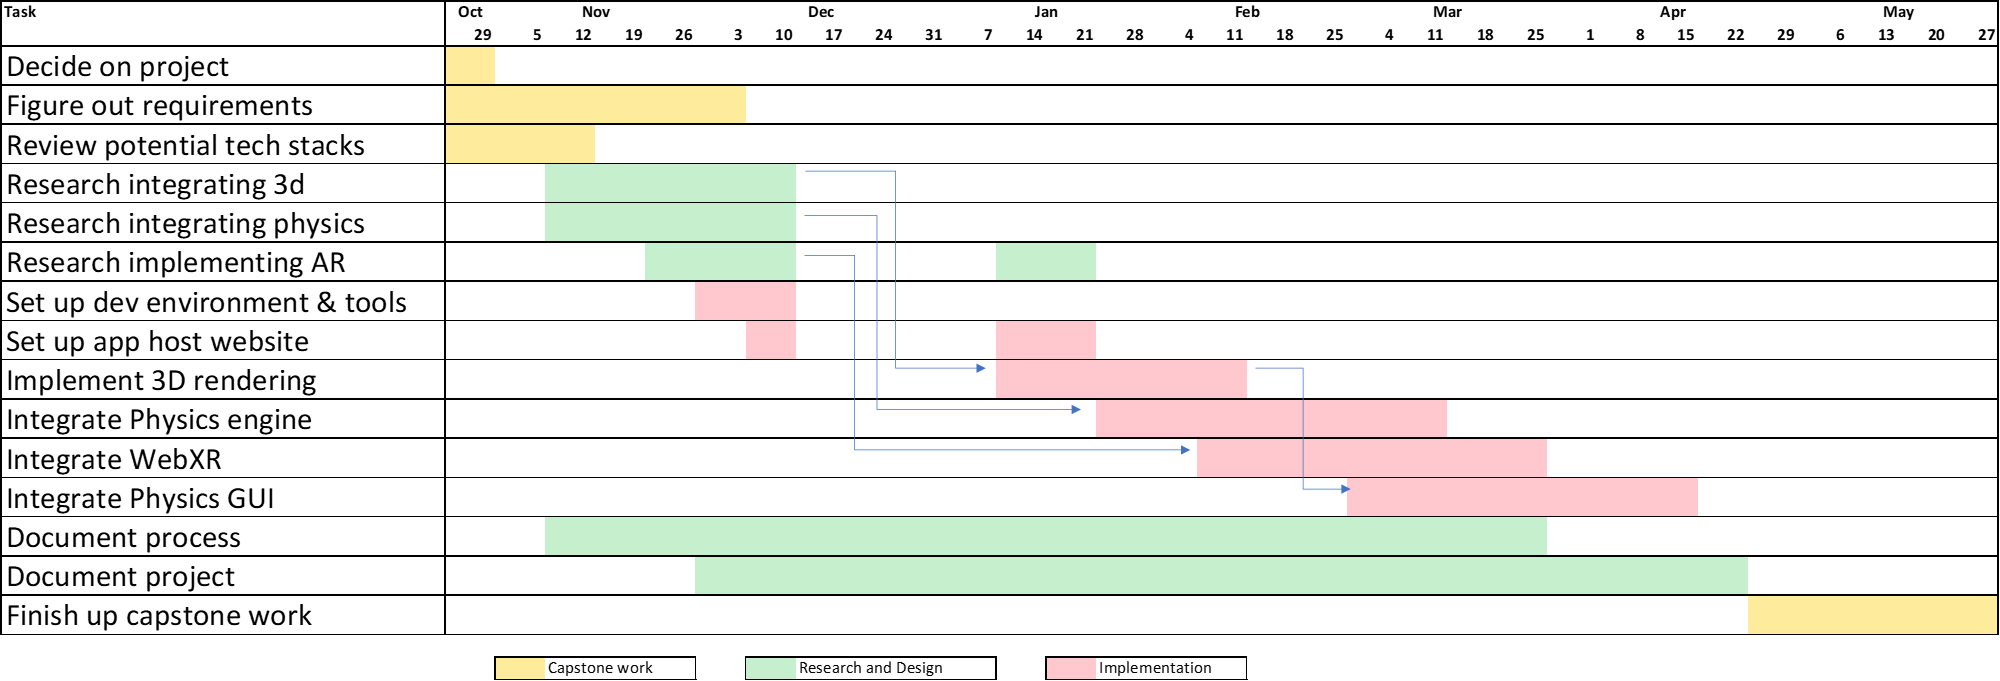
\includegraphics[width=\textwidth]{gantt.png}
\newpage
\bibliographystyle{ieeetr}
\bibliography{sources}

\end{document}
